\subsubsection*{Analysis}
\begin{tabular}{@{}l l}
\textbf{Scope}:&The AuctionHouse\textsuperscript{TM} automated administration system\\
\textbf{Level}:&User goal\\
\textbf{Primary Actor}:&Secretary\\
\textbf{Stakeholders and Interests}:&\begin{tabular}[t]{@{}l}
	Secretary: wants to enter the new customer's parameters easily and quickly.\\
	Customer: wants to be registered as a regular customer.\\
	Search System: wants to have the customers mail address to be added\\\hspace*{5mm}to a mailing list for future reference.\\
	Search System: wants to have the customers e-mail address to be added\\\hspace*{5mm}to a e-mailing list for future reference.\end{tabular}\\
\textbf{Preconditions}:&Secretary is identified and authenticated.\\
\textbf{Postconditions}:&\begin{tabular}[t]{@{}l}
	The customer is registered in the system as a ``regular customer''.\\
	The customer's address has been added to a mailing list for the auction catalogue.\\
	If the customer specified a category of interest, their e-mail address has been\\
	added to a mailing list for the theme-specific notifications.\end{tabular}\\
\textbf{Special requirements}:&A list of item categories/themes is available in the system\\
\textbf{Frequency of occurence}:& \begin{tabular}[t]{@{}l}The total amount or registrnations varies through time. For example, after an\\auction, newer customers may decide they want to visit on a more regular basis.\\On average, 5 to 10 customers register every month.\footnotemark\end{tabular}
\end{tabular}\\\\
\footnotetext{The numbers came from a contact session with John. Session details are in the references, page \pageref{conv2}}
\textsl{Main Success Scenario}
\begin{enumerate}[noitemsep]
	\item The user starts the `register regular customer' transaction with the system, having all parameters of the item to be added ready.
	\item The system returns a list of item categories.
	\item The user provides the following information.
	\begin{itemize}[noitemsep]
		\item The customer's name
		\item The customer's address
		\item The customer's postal code
		\item The customer's city data
		\item Category of interest (optional)
		\item The customers e-mail address (required if the above was provided)
	\end{itemize}
	\item The system registers the new regular customer using the provided parameters and generates a customer ID.
	\item The system adds the provided address to the mailing list
	\item If a category of interest was provided, the system adds the the provided e-mail address to the e-mailing list of that category.
	\item The system returns to the user with a confirmation message containing the generated customer ID. 
\end{enumerate}
\textsl{Extensions}
\begin{itemize}[noitemsep]
	\item 3a. When not all required parameters were provided, the system will not register the user, but notify the user of this error and ask them to provide it before continuing.
	\item 6a. If the user chooses a category of interest, but does not provide an e-mail address, the system will not register the user, but notify the user of this error and ask them to provide it before continuing.
\end{itemize}
\newpage
\textsl{System Sequence Diagram}
\begin{figure}[H]
	\centering
	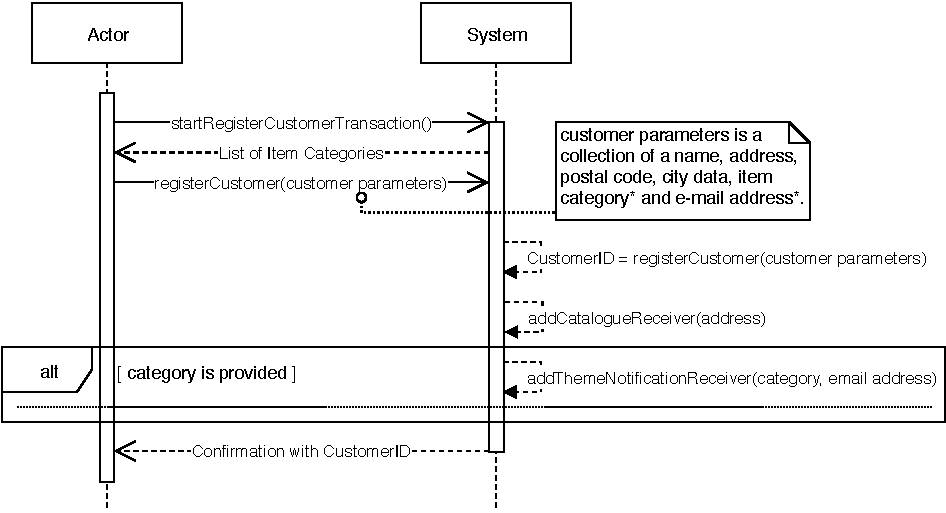
\includegraphics[scale=1]{uml/SD-bb-regcust.pdf}
	\caption*{Interactions displayed in a System Sequence Diagram defined by the MSS and its extensions in blackbox format. Paramters marked with a `*' are optional and can be omitted.}
\end{figure}
\newpage
\textsl{Glossary}
\begin{center}\begin{tabular}{l|l}
\textbf{Function}&\textbf{Clarification}\\\hline\hline
startRegisterCustomerTransaction()&\begin{tabular}[t]{@{}l}Starts the `register customer' transaction with the system.\end{tabular}\\\hline
registerCustomer(customer parameters)&\begin{tabular}[t]{@{}l}Requests the system to register a regular customer, to be created\\from the provided parameters. This request will \underline{not} register the\\regular customer in the system. Therefore, this request can return\\a failure, leaving the system state unchanged.\end{tabular}\\\hline
getPaymentStatus(customer)&\begin{tabular}[t]{@{}l}Gets the payment status of the customer who wants to register\\a search request. Result can be ``Paid'' or ``Not Paid''.\end{tabular}\\\hline
createCustomer(request parameters)&\begin{tabular}[t]{@{}l}Creates a new regular customer from provided parameters and\\registers it to the search system. Returns the id of the new\\regular customer.\end{tabular}\\\hline
addCatalogueReceiver(address)&\begin{tabular}[t]{@{}l}Adds the provided address to a Mailing List so the catalogue will\\(from now on) also be sent to this address.\end{tabular}\\\hline
\begin{tabular}[t]{@{}l}addThemeNotificationReceiver(\\category, e-mail address)\end{tabular}&\begin{tabular}[t]{@{}l}Adds the provided e-mail address to a E-Mailing List for the\\specified category so an e-mail notification related to this category\\will (from now on) also be sent to this e-mail address.\end{tabular}
\end{tabular}\end{center}